%%%%%%%%%%%%%%%%%%%%%%%%%%%%%%%%%%%%%%%%%%%%%%%%%%%%%%%%%%%%%%%%%%%%%%%%%%%%%
%
%  System        : 
%  Module        : 
%  Object Name   : $RCSfile$
%  Revision      : $Revision$
%  Date          : $Date$
%  Author        : $Author$
%  Created By    : Robert Heller
%  Created       : Thu May 20 07:35:55 2021
%  Last Modified : <210520.0859>
%
%  Description 
%
%  Notes
%
%  History
% 
%%%%%%%%%%%%%%%%%%%%%%%%%%%%%%%%%%%%%%%%%%%%%%%%%%%%%%%%%%%%%%%%%%%%%%%%%%%%%
%
%    Copyright (C) 2021  Robert Heller D/B/A Deepwoods Software
%			51 Locke Hill Road
%			Wendell, MA 01379-9728
%
%    This program is free software; you can redistribute it and/or modify
%    it under the terms of the GNU General Public License as published by
%    the Free Software Foundation; either version 2 of the License, or
%    (at your option) any later version.
%
%    This program is distributed in the hope that it will be useful,
%    but WITHOUT ANY WARRANTY; without even the implied warranty of
%    MERCHANTABILITY or FITNESS FOR A PARTICULAR PURPOSE.  See the
%    GNU General Public License for more details.
%
%    You should have received a copy of the GNU General Public License
%    along with this program; if not, write to the Free Software
%    Foundation, Inc., 675 Mass Ave, Cambridge, MA 02139, USA.
%
% 
%
%%%%%%%%%%%%%%%%%%%%%%%%%%%%%%%%%%%%%%%%%%%%%%%%%%%%%%%%%%%%%%%%%%%%%%%%%%%%%

\chapter{ESP32-PWMHalfSidingSMD: Half Siding board base board for an ESP32 Dev Kit MCU board}

This is a circuit board that supports an ESP32 Dev Kit board or TTGO-T1 board 
to manage one half (one end) of a siding.  This board can also be used to 
manage two bi-directional single track ABS blocks or one bi-directional dual 
track ABS block.  There are other trackwork cases this board can handle as 
well.  The board contains these I/O sections:

\begin{itemize}
\item Two occupancy detectors.  These are optoisolator based, so they will 
work for both DC and DCC systems.
\item Two stall-motor with point sense.
\item Sixteen PWM Led drivers.  These are meant to light lamps in signal 
heads.
\end{itemize}

This board uses six GPIO pins and one I2C channel:

\begin{description}
\item[GPIO0] Motor Select 1: select the position of stall motor 1.
\item[GPIO12] Motor Select 2: select the position of stall motor 2.
\item[GPIO34] Point Sense 1: return the state of the points for 
stall motor 1. 
\item[GPIO35] Point Sense 2: return the state of the points for 
stall motor 2. 
\item[GPIO26] Occupancy Detector 1.
\item[GPIO27] Occupancy Detector 2.
\item[GPIO16] (Optional) Output enable for the PWM LED Controller.
\item[I2C Address 0x40] A PCA9685 16-channel, 12-bit PWM LED Controller.
\end{description}

Each of the motor drive circuits is through a TC4428, which can drive up to
1.5A, which is way more needed to drive a typical stall motor. It is enough to
drive a pair of stall motors, wired in parallel as would be the case for a
cross over. 

\section{Circuit Description}


\subsection{Turnout Control}
\begin{figure}[hbpt]\begin{centering}%
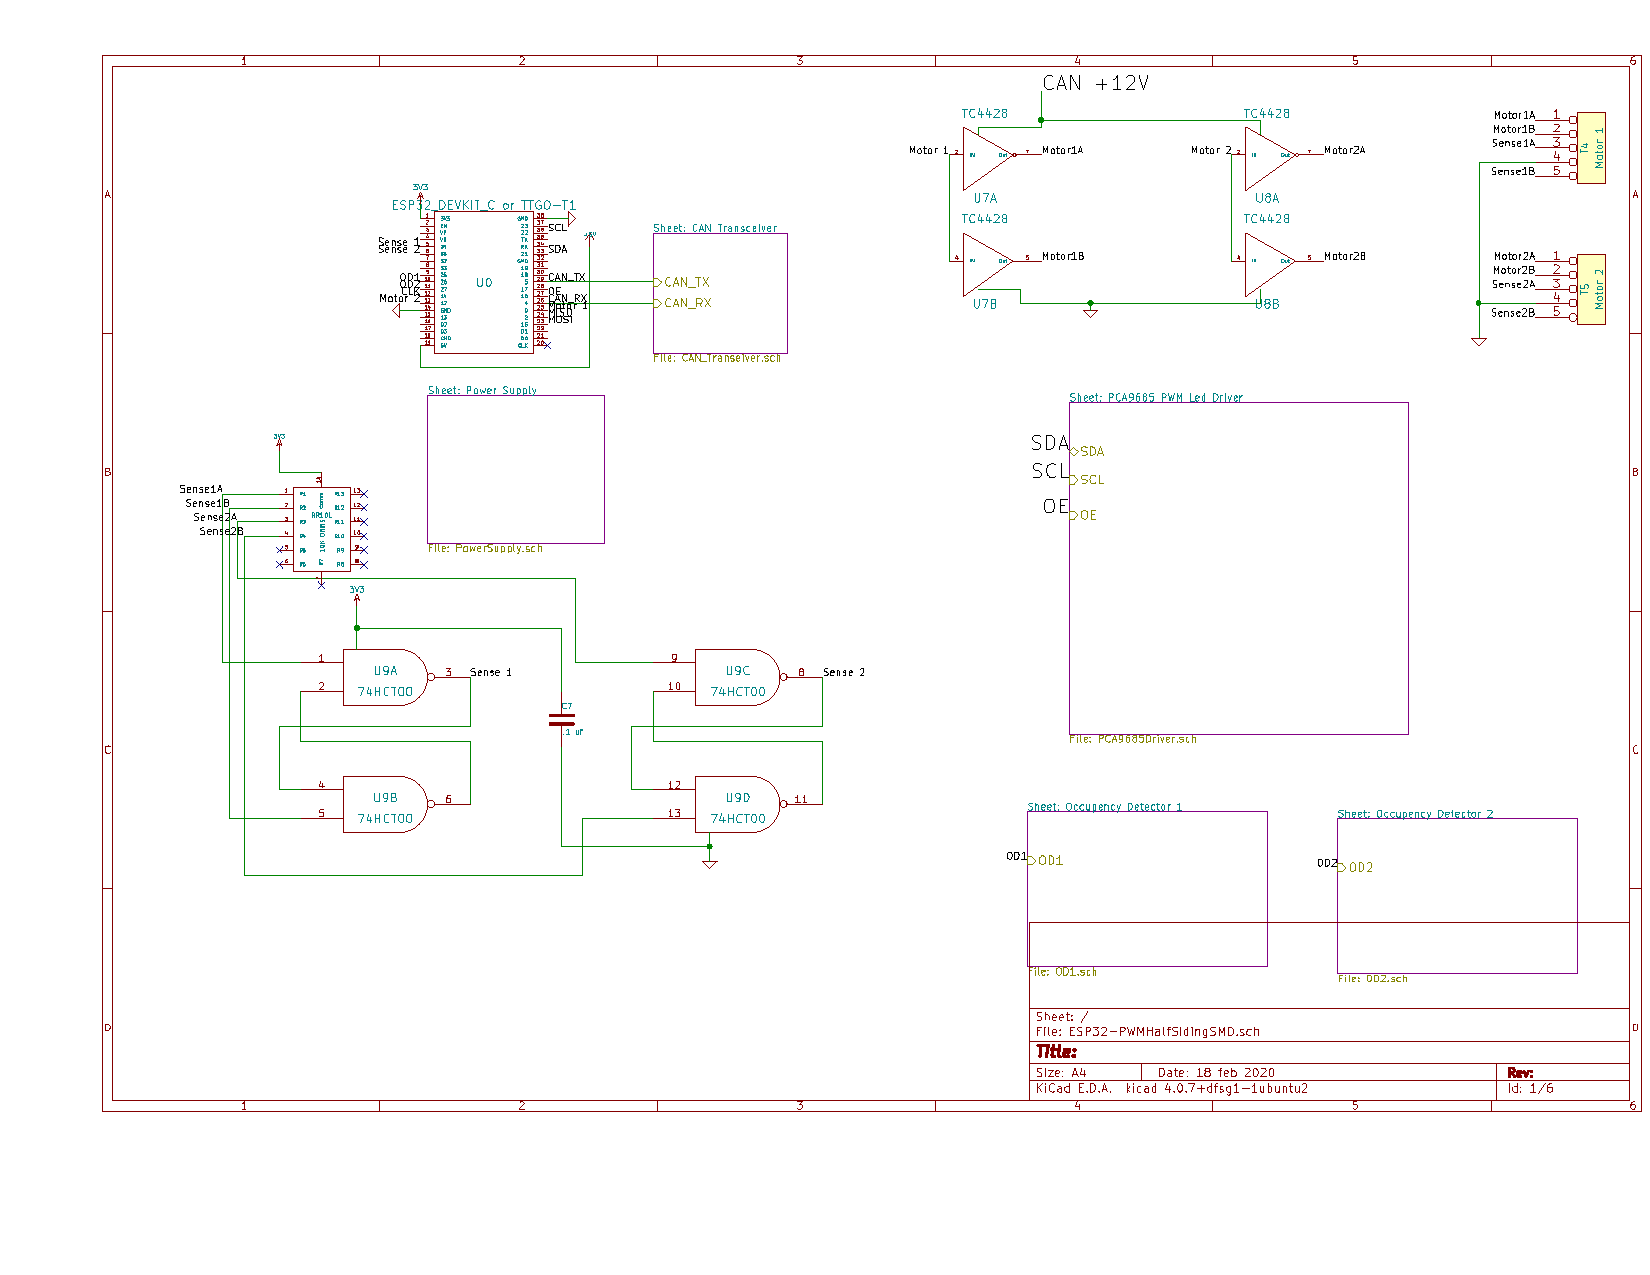
\includegraphics[width=5in]{ESP32-PWMHalfSidingSMD-1.pdf}
\caption{Circuit Diagram of the ESP32-PWMHalfSidingSMD, page 1 (ESP32 MCU and 
Turnout Driver and Sense)}
\end{centering}\end{figure}

The turnout control has two parts. There is an output section that contains
two TC4428 chips. Each chip has a non-inverting and an inverting driver. The
inputs of both drivers are connected to one of the motor GPIO pins. The output
are wired to the terminal block for a one of the motors. For any given logic
state of the motor control output, one of the drivers is ``on'' and the other
is ``off'', thus one motor terminal is ground and one is raised to the 12V
supply. This means alternative states of the logic line will drive the stall
motor in alternative directions. 

The other section is a pair of flip-flop debounce circuits, one for each of
two SPDT switch contacts that report the position of the turnout points. The
output of these flip-flops goes to a pair of GPIO input pins.

\clearpage
\subsection{CAN Transceiver}
\begin{figure}[hbpt]\begin{centering}%
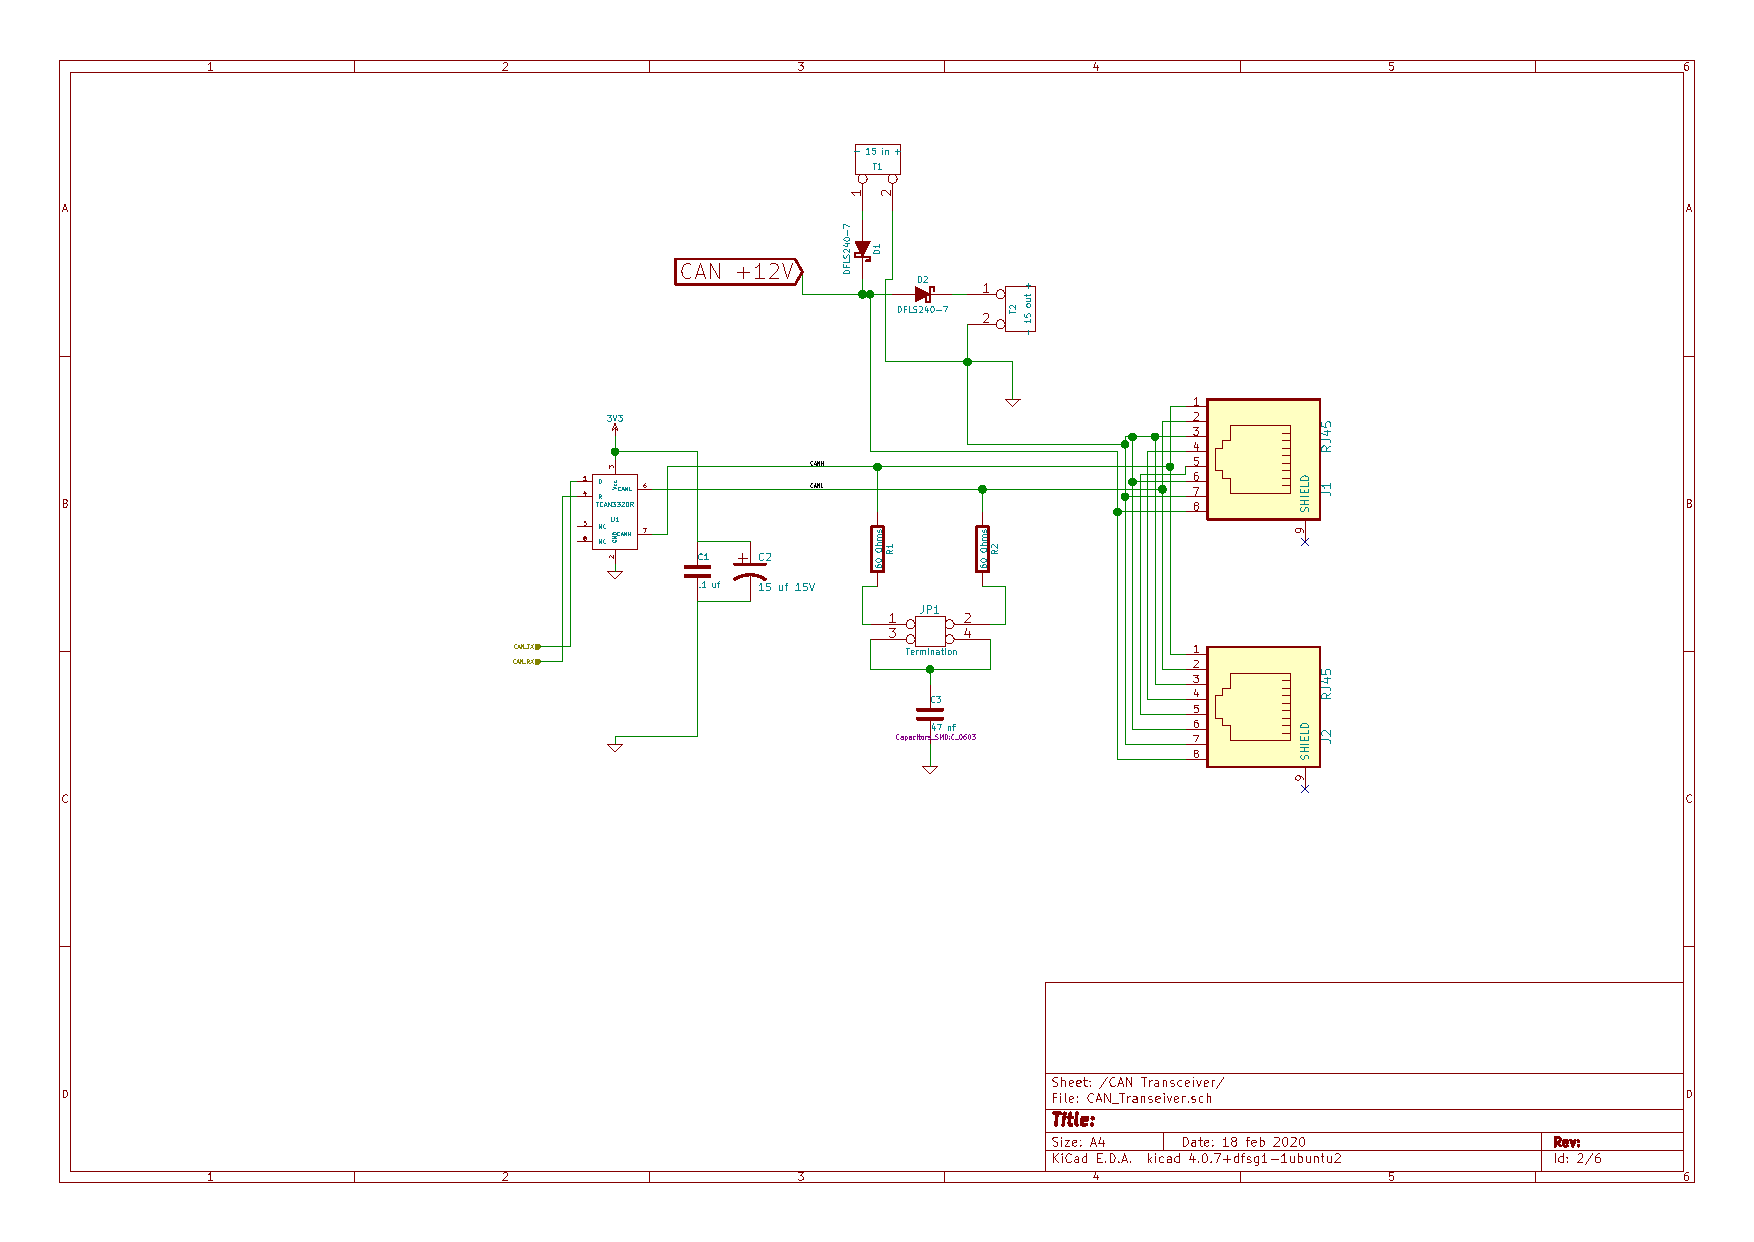
\includegraphics[width=5in]{ESP32-PWMHalfSidingSMD-2.pdf}
\caption{Circuit Diagram of the ESP32-PWMHalfSidingSMD, page 2 (CAN Transceiver)}
\end{centering}\end{figure}

This section contains the CAN Transceiver, along with a termination jumper 
block. Power insertion and pick off and the RJ45 Jacks.

\clearpage
\subsection{Power Supply}
\begin{figure}[hbpt]\begin{centering}%
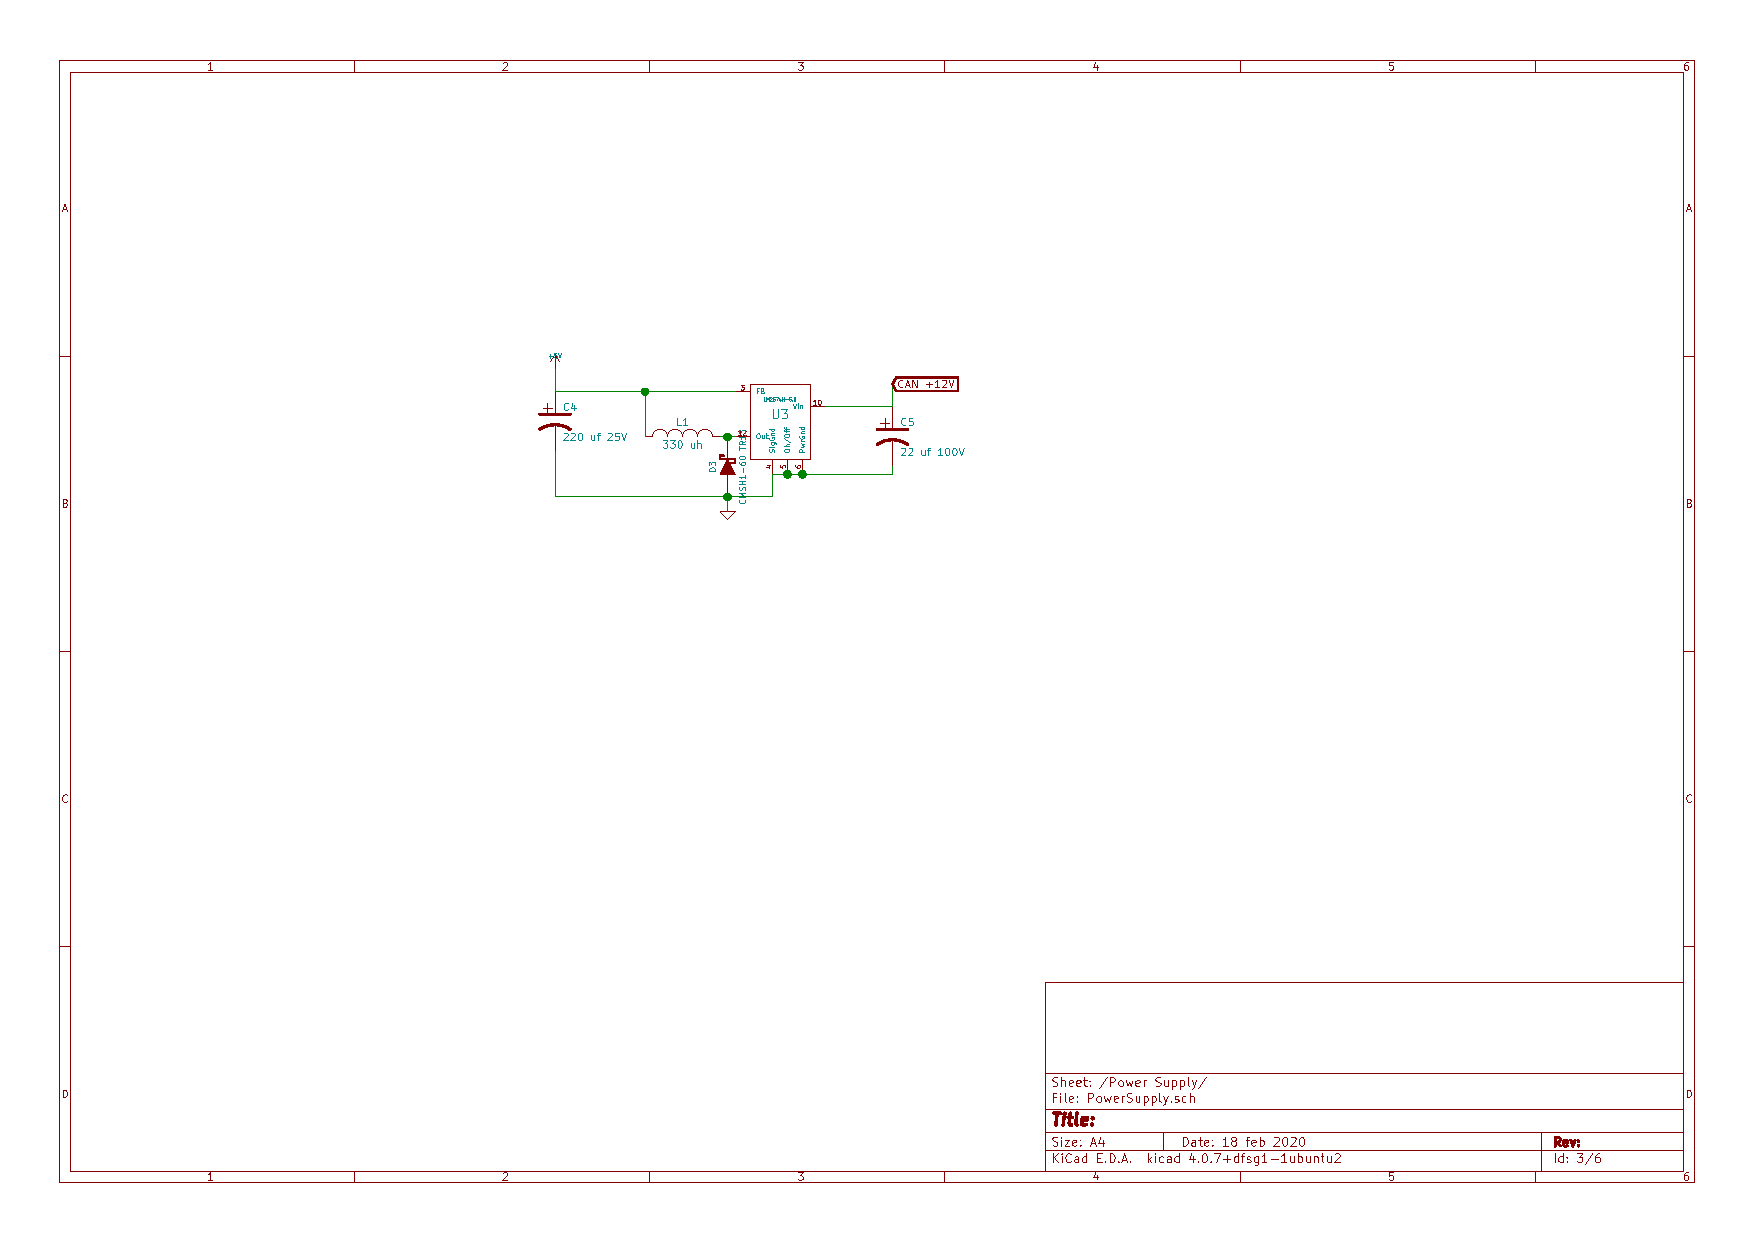
\includegraphics[width=5in]{ESP32-PWMHalfSidingSMD-3.pdf}
\caption{Circuit Diagram of the ESP32-PWMHalfSidingSMD, page 3 (Power Supply)}
\end{centering}\end{figure}

This section contains a 5V power supply that takes the nominal 12V on the CAN 
power bus and regulates it down to 5V to supply the ESP32 MCU board.

\clearpage
\subsection{Occupancy Detectors}
\begin{figure}[hbpt]\begin{centering}%
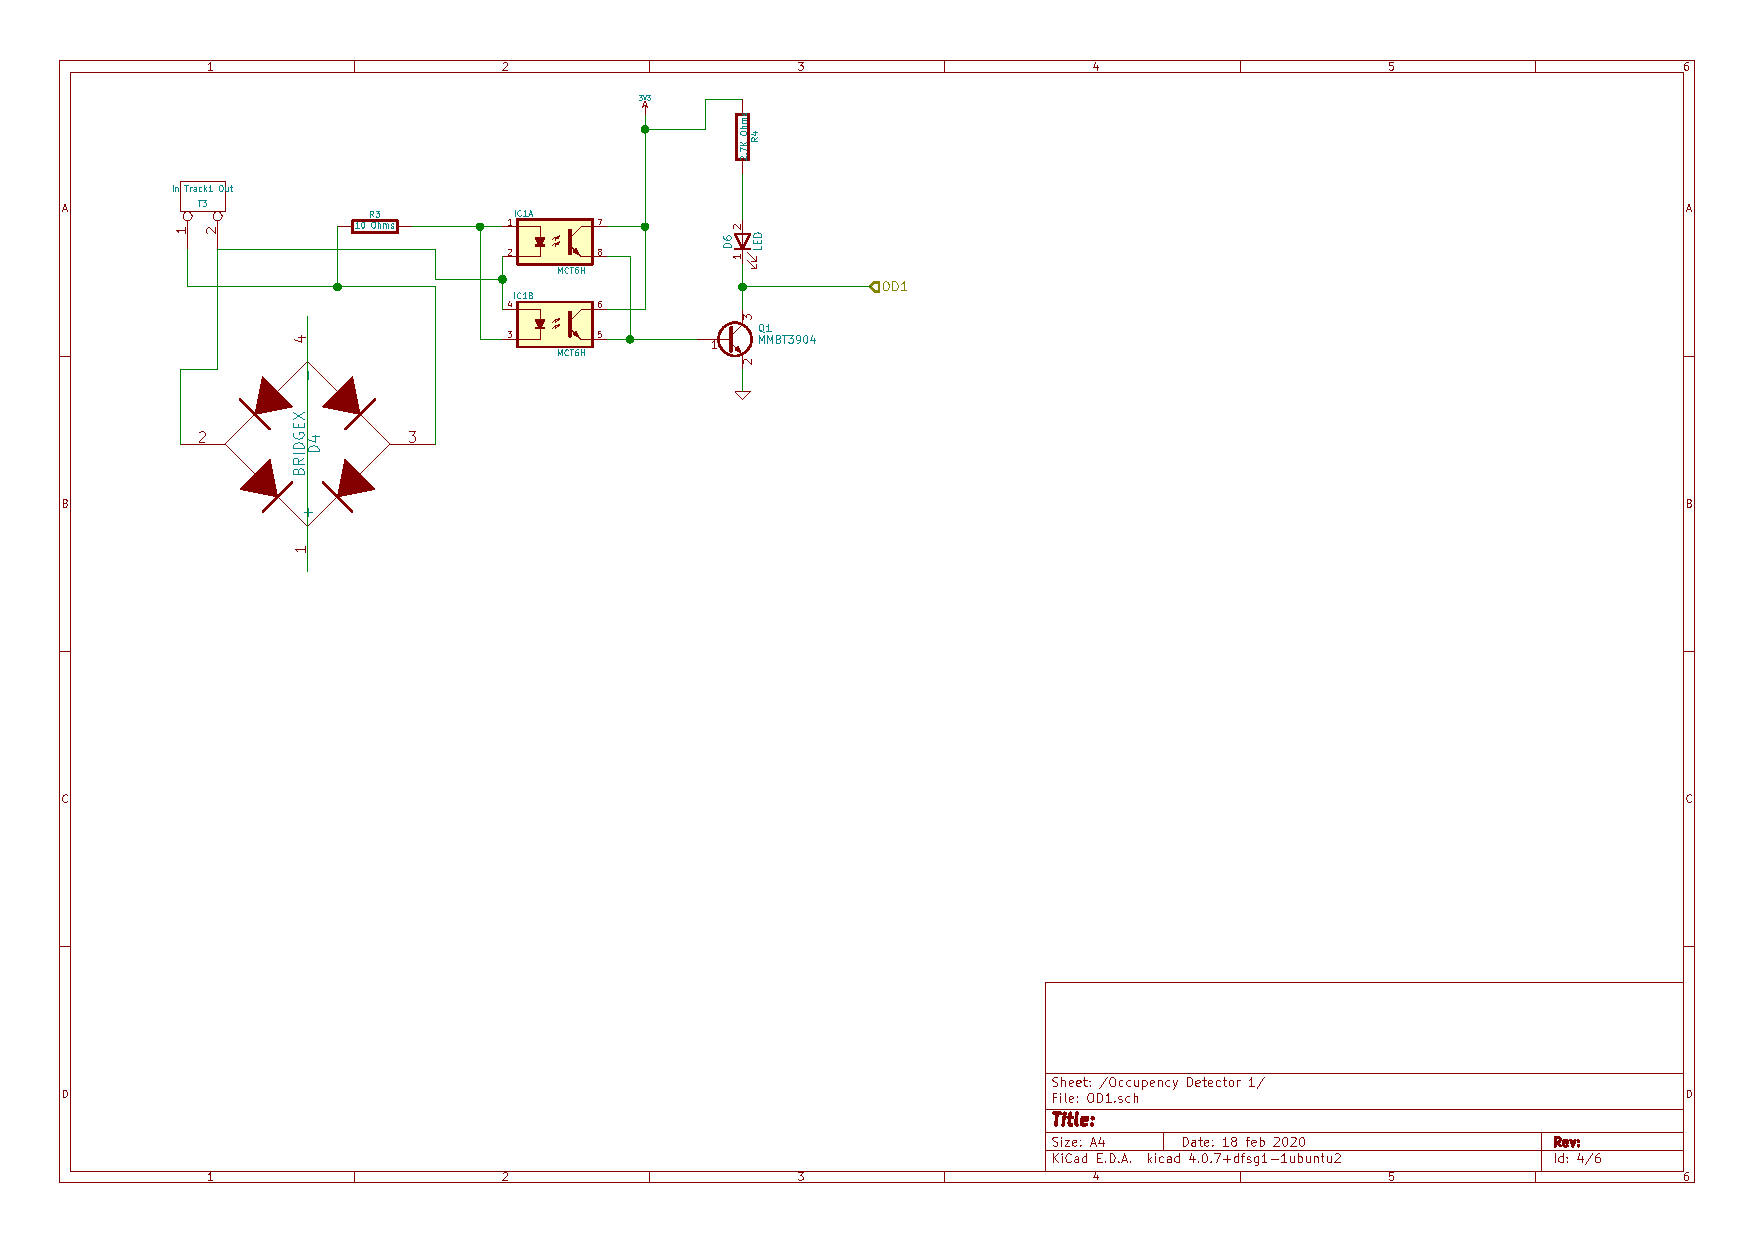
\includegraphics[width=5in]{ESP32-PWMHalfSidingSMD-4.pdf}
\caption{Circuit Diagram of the ESP32-PWMHalfSidingSMD, page 4 (Occupancy 
Detector 1)}
\end{centering}\end{figure}
\begin{figure}[hbpt]\begin{centering}%
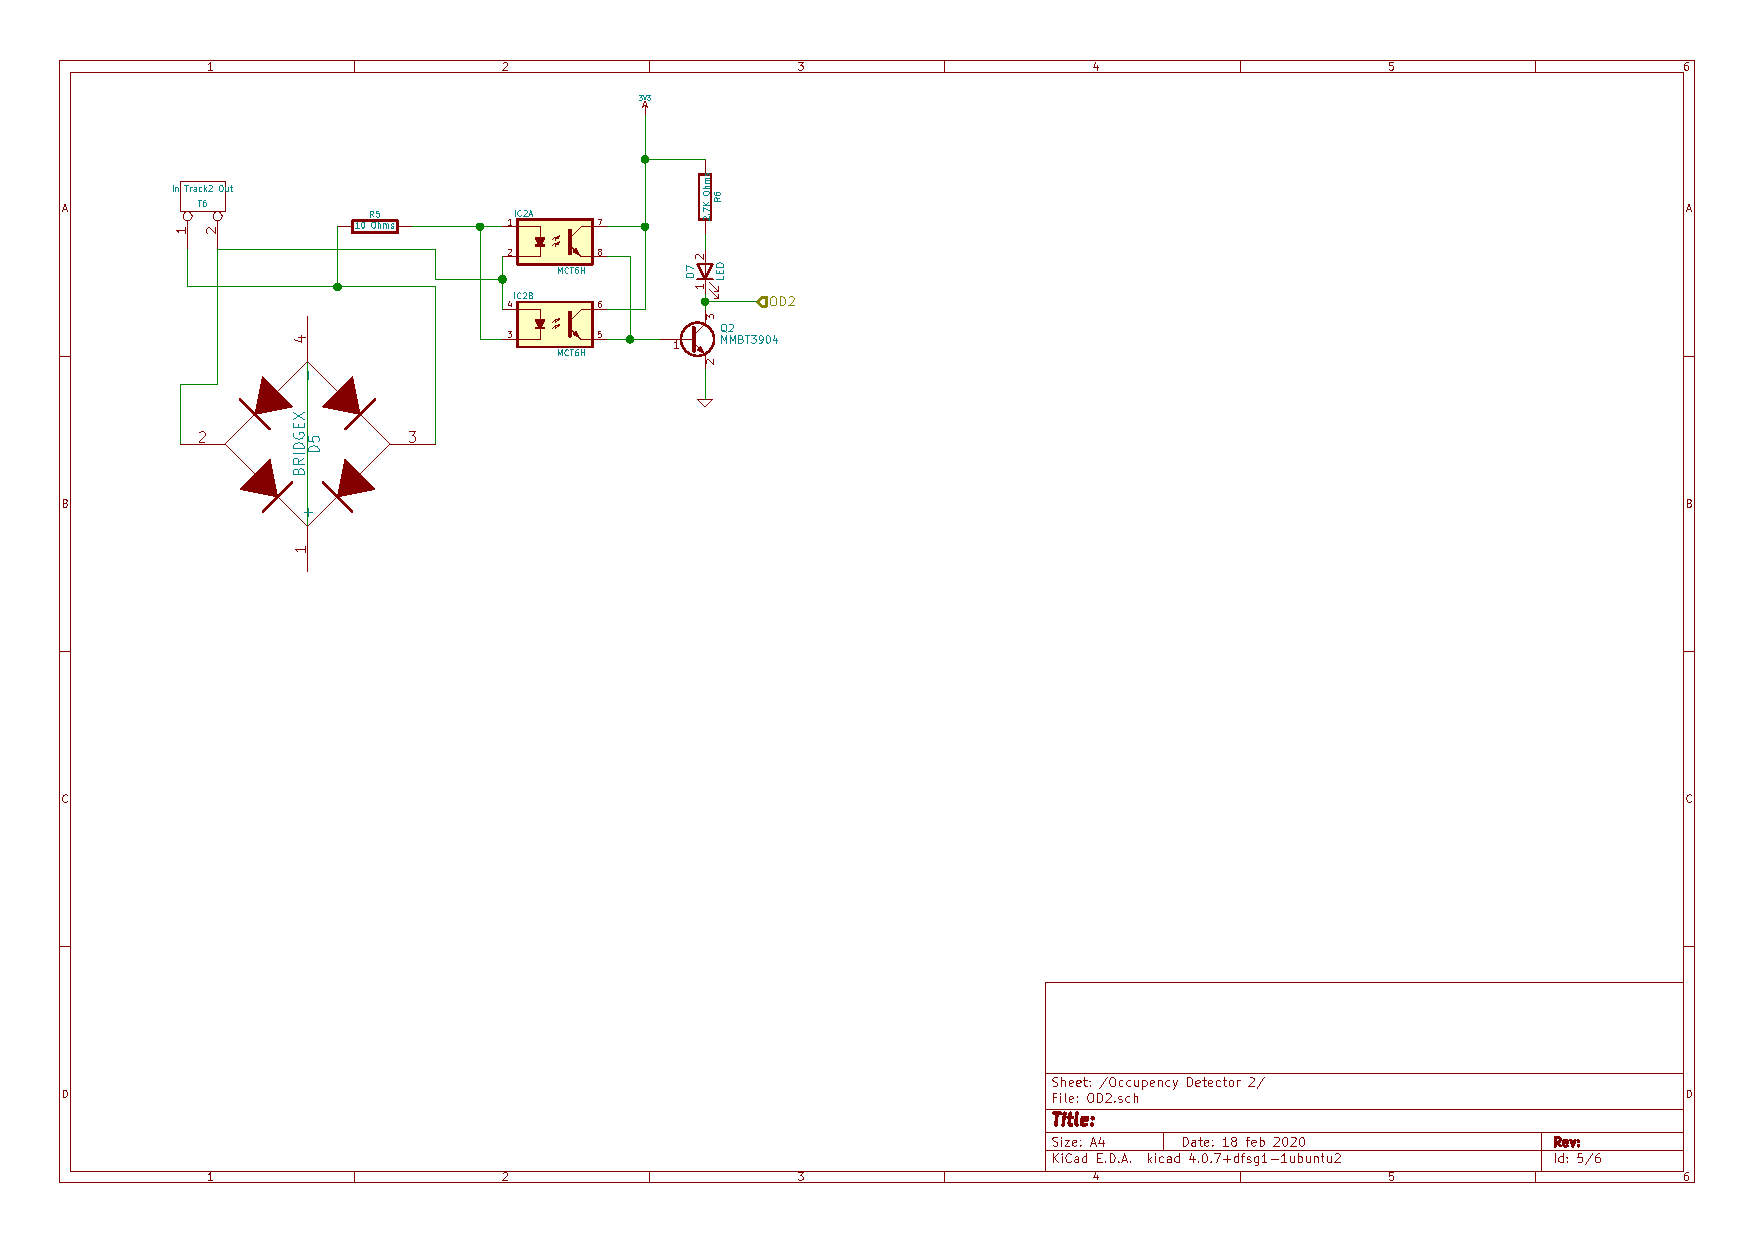
\includegraphics[width=5in]{ESP32-PWMHalfSidingSMD-5.pdf}
\caption{Circuit Diagram of the ESP32-PWMHalfSidingSMD, page 5 (Occupancy 
Detector 2)}
\end{centering}\end{figure}

The occupancy detectors use optoisolators in series with the track power 
supply.  There is a heavy duty bridge rectifier in parallel with the 
optoisolators to carry the bulk of the current to the track.  They will work 
with either DC or DCC track power.

\clearpage
\subsection{PWM LED Driver}
\begin{figure}[hbpt]\begin{centering}%
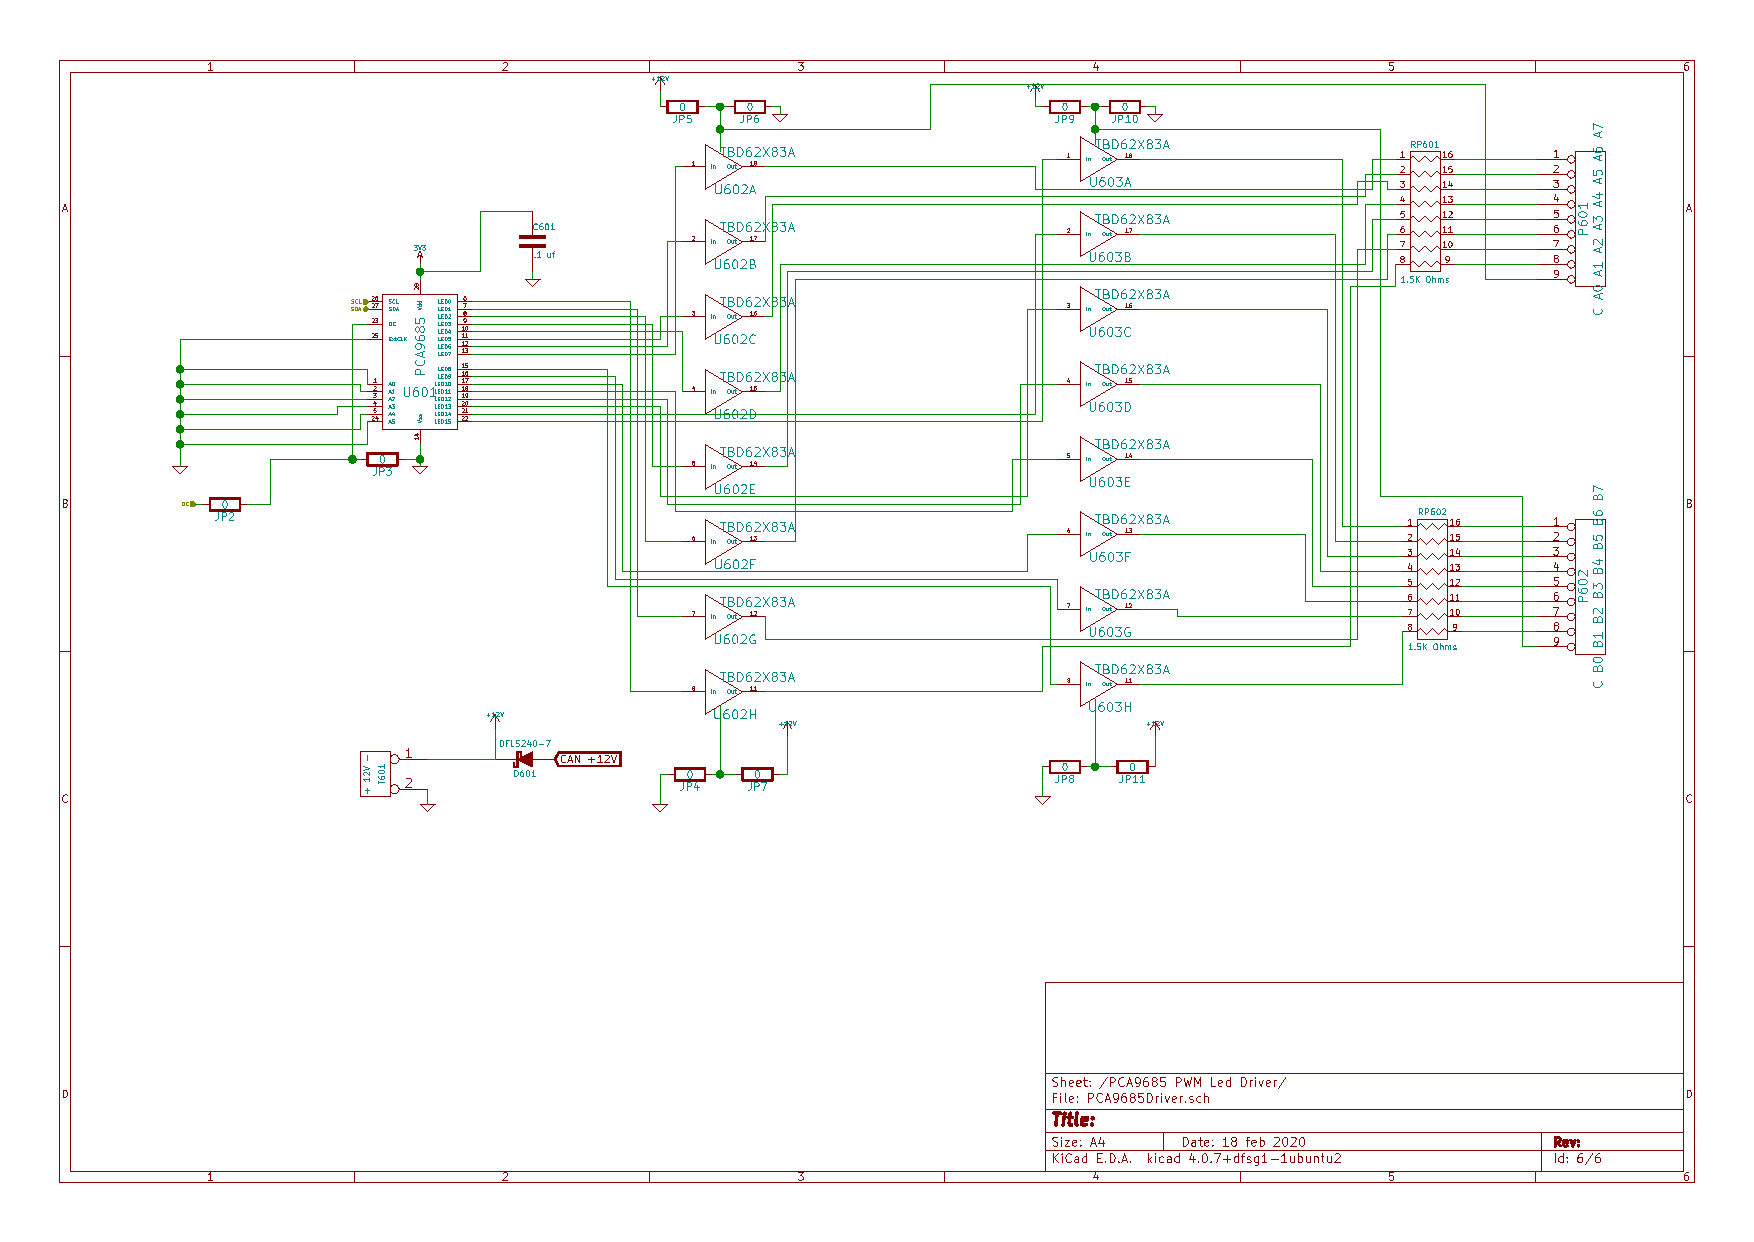
\includegraphics[width=5in]{ESP32-PWMHalfSidingSMD-6.pdf}
\caption{Circuit Diagram of the ESP32-PWMHalfSidingSMD, page 6 (PWM LED Driver)}
\end{centering}\end{figure}

The PWM LED Driver uses a PCA9685 which is a 16 channel, 12 bit PWD LED 
driver.  A pair of octal MOSFET drivers and series load resistors are also 
included on the board.  The MOSFET drivers come in both inverting (low-side 
drive) and non-inverting (high-side drive), so it is possible to support both 
common anode and common cathode LED signals.

\clearpage
\section{User Installed Parts}

\begin{centering}\begin{tabular}{|r|l|l|p{1.5in}|p{1.5in}|}
\hline
Index&Qty&Refs&Mouser Part Number&Description\\   
\hline
1&2&J1, J2&710-615008144221&RJ45 Jacks\\
\hline
2&1&JP1&649-67997-404HLF&Termination Jumper\\
\hline
3&2&P601, P602&651-1725724&Signal Lamp Terminals\\
\hline
4&3&T1, T2, T601&651-1725656&LCC and Signal power\\
\hline
5&2&T3, T6&490-TB007-508-02BE&Occupancy Terminals\\
\hline
6&2&T4, T5&651-1725685&Turnout terminals\\
\hline
7&2&U0&517-929974-01-19-RK&MCU Headers\\
\hline
8&1&U0&517-929850-01-18-10&MCU Headers\\
\hline
\end{tabular}\end{centering}
